\documentclass[../main.tex]{subfiles}

\begin{document}

This part of the document is written from another file. However, it is not necessary to reimport the packages loaded in the main document: \LaTeX{} does it for us. For example, \texttt{mathtools} is correctly loaded \[ x \coloneqq \frac{-b \pm \sqrt{b^2-4ac}}{2a} \]

And obviously, you can import images the same way

\begin{figure}
    \centering
    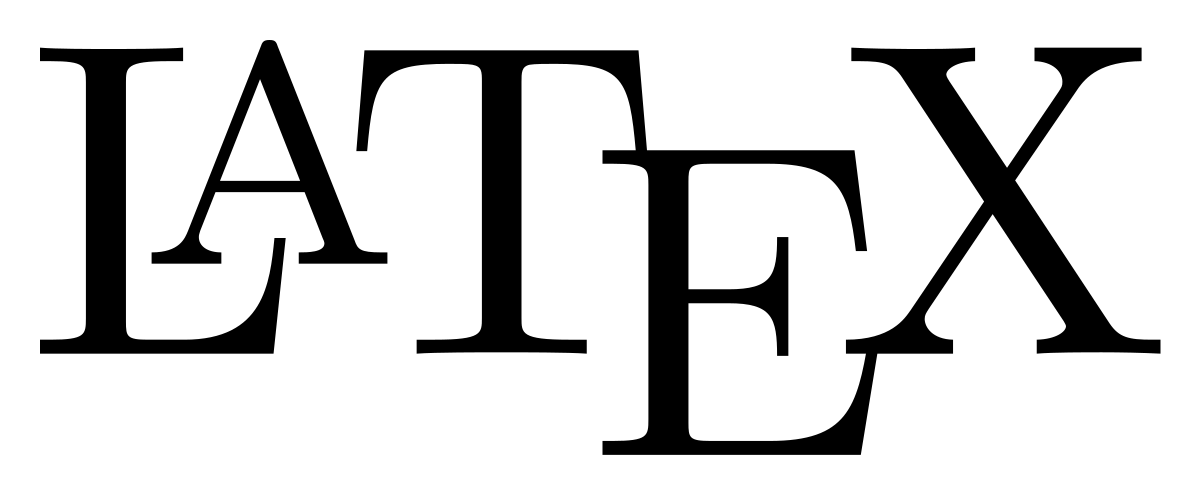
\includegraphics[width=3cm]{LaTeX}
    \caption{An example of image integration from a subfile}
\end{figure}

\begin{theorem}[Don't repeat yourself]
Everything that is declared in \texttt{main.tex} can be reused here (like this theorem environment).
\end{theorem}

\end{document}
